\chapter{他のソフトとの比較}\label{ux4ed6ux306eux30bdux30d5ux30c8ux3068ux306eux6bd4ux8f03}

    他のタイピングソフトとの比較を行った表が以下の通りである.

\begin{table}[H]
\centering
\begin{center}
\caption{他のソフトとの比較.\label{compare}}
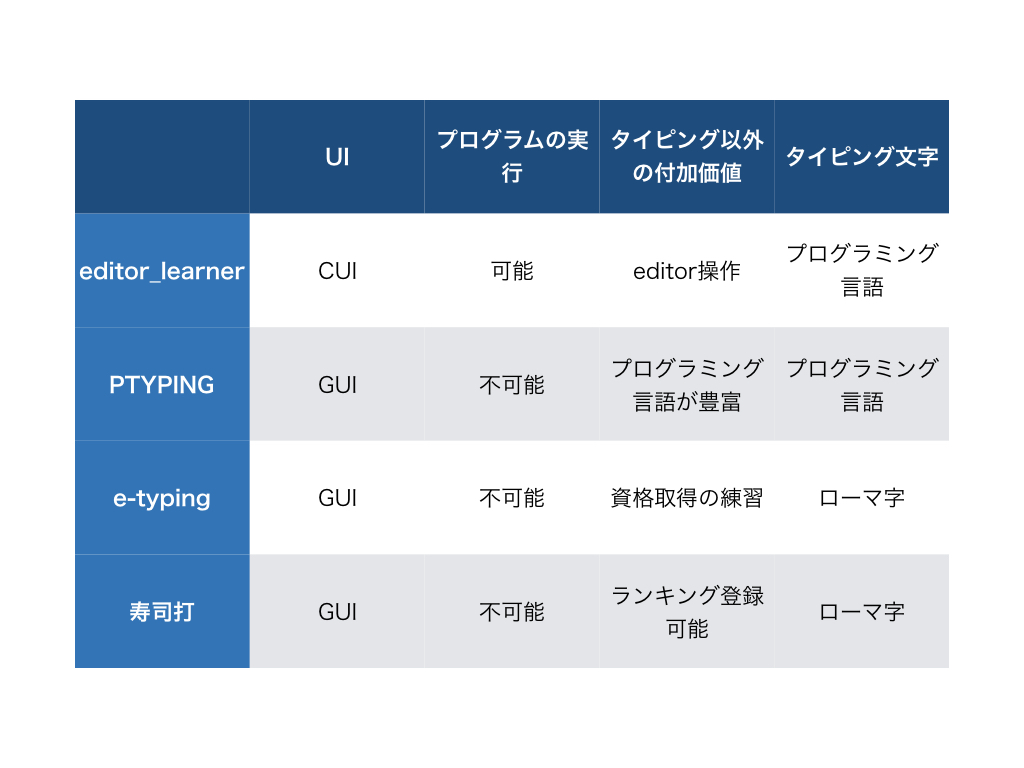
\includegraphics[width=150mm]{../../picture/compare.jpeg}
\end{center}

\label{fig:}
\end{table}

上記のタイピングソフトは自分もよく使っていたタイピングソフトであり,評価も高いソフトである.それぞれの特徴は以下の通り.

\begin{enumerate}
\def\labelenumi{\arabic{enumi}.}
\tightlist
\item
PTYPING: 豊富なプログラミング言語がタイピング可能
\item
e-typing: 資格取得にもつながる練習が可能.間違いが多い箇所を指摘してくれる.
\item
寿司打: 自分が一番よく使ったソフト,GUIベースで飽きずに継続しやすい.
\end{enumerate}

それぞれの特徴があるが,人気ソフトの中でもプログラムの実行が可能なソフトは発見できなかった.プログラマにとってコードを書いて実行しないのは,テストを受けて結果を見ないのと同義である.また,これらのソフトは全てWeb上で行なっており,editorは全く使わない.プログラマにとってコードだけ書いてeditorを使って実行しないことなどない.よっていかにeditor\_learnerがプログラマ向けのソフトかがわかる.

\section{考察}\label{ux8003ux5bdf}

editor\_learnerは様々な機能を有しており,\{\}や()などの約物の記入,editor操作やプログラムの実行などが可能な点であり,editor操作によるキーバインドの習熟が期待される.

GUIベースのソフトに比べて継続性では劣るが,CUIベースのeditor\_learnerではファイルの保存,開閉による操作を習熟することができ作業を効率化,高速化することができる.これらの理由によりeditor\_learnerでは目的に沿った技術の向上が期待される.

    